\documentclass[a4paper,12pt]{article}

\usepackage{graphicx}
\usepackage[top=1in, left=0.9in, right=1.25in, bottom=1in]{geometry}
\usepackage[utf8]{inputenc}
\usepackage{float} % Etiqueta 'H' (mayus) en figuras (imágenes)
\usepackage{array} % Padding en tablas
\usepackage{url} % Etiqueta url en .bib
\usepackage{booktabs} % Manejo de caudros (tablas)
\usepackage[T1]{fontenc}    % Codificación de fuentes
\usepackage{csquotes}       % Paquete para comillas tipográficas
\usepackage[spanish,es-nodecimaldot,es-tabla]{babel}
\usepackage{tikz} 
\usepackage{tocloft}
\graphicspath{{./figs/}}
\usepackage{setspace}

\renewcommand\cftsecpresnum{\S}
\renewcommand\cftsubsecpresnum{\S}  

%------------------------------
\begin{document}

    \begin{titlepage}
        \thispagestyle{empty}
        \begin{minipage}[c][0.17\textheight][c]{0.25\textwidth}
            \begin{center}
                
\includegraphics[width=3.5cm, height=3.5cm]{media/Escudo-UNAM.pdf}
            \end{center}
        \end{minipage}
        \begin{minipage}[c][0.195\textheight][t]{0.75\textwidth}
            \begin{center}
                \vspace{0.3cm}
                \textsc{\large Universidad Nacional Aut\'onoma de M\'exico}\\[0.5cm]
                \vspace{0.3cm}
                \hrule height2.5pt
                \vspace{.2cm}
                \hrule height1pt
                \vspace{.8cm}
                \textsc{Facultad de Ingenier\'ia}\\[0.5cm] %
            \end{center}
        \end{minipage}

        \begin{minipage}[c][0.81\textheight][t]{0.25\textwidth}
            \vspace*{5mm}
            \begin{center}
                \hskip2.0mm
                \vrule width1pt height13cm 
                \vspace{5mm}
                \hskip2pt
                \vrule width2.5pt height13cm
                \hskip2mm
                \vrule width1pt height13cm \\
                \vspace{5mm}
                
\includegraphics[height=4.0cm]{media/ESCUDO-FI_negro.jpg}
            \end{center}
        \end{minipage}
        \begin{minipage}[c][0.81\textheight][t]{0.75\textwidth}
            \begin{center}
                \vspace{1cm}

                {\large\scshape (1317) Estructura de Datos y Algoritmos II }\\[.2in]
                
                \textsc{\large Profesor: M.I. Edgar Tista Garcia}\\[.25cm]
                \textsc{\large Grupo: 05}\\ [.25cm]
                \textsc{\large Semestre 2024-2}\\

                \vspace{1cm}            
 
                \textsc{\large \textbf{Proyecto 1 - Complejidad Computacional en los Algoritmos de Ordenamiento.}}\\[.5cm]
                \textsc{\large \textbf{Documentación}}\\[1cm]
                \textsc{\large Equipo 02}\\ [1cm]
                \textsc{\large Integrantes:}\\[0.25cm]
                \textsc{\large Cabrera Rojas Oscar}\\[0.25cm]
                \textsc{\large Chavez Marquez Sergio Antonio}\\[0.25cm]
                \textsc{\large {Noyola Torres Pablo Sebastian}}\\[2cm]          


                \vspace{0.5cm}
                \textsc{\large Lunes 25 de marzo del 2024}\\[0.25cm]
            \end{center}
        \end{minipage}
    \end{titlepage}

\section{Material de apoyo}

Para la investigación del algoritmo de ordenamiento adicional y la escritura de archivos en Java, consultó los siguientes sitios en internet en su búsqueda confiable de información.

\subsection{API de Java}

\begin{itemize}
    \item Oracle. (2014). \textit{Class FileWriter}. Java Platform Standard Edition 8 Documentation. Recuperado 22 de marzo de 2024, de\\https://docs.oracle.com/javase/8/docs/api/java/io/FileWriter.html
    \item Oracle. (2014). \textit{Class IOException}. Java Platform Standard Edition 8 Documentation. Recuperado 22 de marzo de 2024, de\\https://docs.oracle.com/javase/8/docs/api/java/io/IOException.html
\end{itemize}

\subsection{Sitios de internet consultados}

\begin{itemize}
    \item \textit{Pancake sorting}. (2023, 11 abril). GeeksforGeeks. Recuperado 22 de marzo de 2024, de https://www.geeksforgeeks.org/pancake-sorting/
    \item Jindal, H. (2023, 12 octubre). \textit{Ordenamiento de panqueques}. DelftStack. Recuperado 21 de marzo de 2024, de https://www.delftstack.com/es/tutorial/algorithm/pancake-sort/
    \item Mario Storti. (2009, 13 noviembre). \textit{Pancake sort algorithm, visualization with VTK} [Vídeo]. YouTube. https://www.youtube.com/watch?v=kk-\_DDgoXfk
    \item The Hexagon. (2023, 11 mayo). \textit{Pancake sort} [Vídeo]. YouTube.\\https://www.youtube.com/watch?v=kXKkHRQmL6o
    \item \textit{Calculadora gráfica - GeoGebra}. (s.f.). https://www.geogebra.org/graphing?lang=es
\end{itemize}

\section{Propuesta de diseño de clases}

Una vez se decidió realizar el programa principal utilizando el lenguaje de programación Java, el diseño y estructura de cada uno de los programas desarrollados resultó ser claro, pues se partió de la idea de implementar una clase individual para cada algoritmo de ordenamiento y, al ser nueve ordenamientos\footnote{Los ordenamientos obligatorios en los requerimentos, el extra y ambos opcionales: \textit{InsertionSort}, \textit{SelectionSort}, \textit{BubbleSort}, \textit{PancakeSort}, \textit{QuickSort}, \textit{HeapSort}, \textit{MergeSort}, \textit{CountingSort} y \textit{RadixSort}.} se requerían entonces nueve archivos destinados a ordenamientos, dichos archivos una vez desarrollados no tienen más acción dentro del funcionamiento general del programa, por lo que lo sería conveniente anexarlos en una carpeta donde puedan guardarse sin contaminar la vista del resto de elementos del programa. Dado el contexto de estar trabajando en Java y retomando la idea de que, para separar física y lógicamente una parte del funcionamiento de un programa se debe conjuntar en un \textit{package}, se decidió también entonces organizar el resto del funcionamiento del programa en paquetes acordes a la lógica de la función de cada programa.

Cada uno de los algoritmos cuenta con un método de partida, generalmente se nombraron exacatamente igual que su clase, con la diferencia de tener la primera letra en minúscula; en el caso de aquellos que funcionan en base a la recursividad (\textit{QuickSort}, \textit{MergeSort} y \textit{PancakeSort}), como estos métodos están guardados en su propia lógica para aplicar la recursividad, su método de inicio se llama \textit{iniciarQuickSort}, \textit{iniciarMergeSort} y \textit{pancakeSortBegin} respectivamente. Estos métodos de inicio son los únicos que contienen un valor de retorno (el de conteo de operaciones)\footnote{En el caso de los algoritmos con recursividad implicada se tuvo que hacer un método distinto al recursivo para el valor de retorno ya que, de funcionar como el resto, el análisis de complejidad se veia comprometido, no funcionando correctamente ni como era esperado.}. Absolutamente todos los métodos implicados en la lógica individual de cada ordenamiento son métodos estáticos, ésto con la idea de que no se van a instanciar objetos de estas clases, sino están destinados única y meramente a realizar su funcionamiento de ordenar un conjunto de datos a la vez.

El contador de operaciones en todos los casos se manejó como una variable de clase para que pueda ser accesible y global para cada parte del funcionamiento, no siendo relevante el lugar de procedencia del incremento.\\

Partiendo de la lógica de lo que debe ser capaz de realizar el programa, se creó lo que es el punto de partida y programa principal, el archivo \textit{Ordenamientos.java}, cuya función es la de ejecutar todos los ordenamientos el número requerido de veces y manejar dichos datos para las operaciones necesarias, éstas son la impresión en pantalla de las tablas correspondientes y la llamada al archivo \textit{Archivos.java} para permitir la correcta graficación de los datos obtenidos y visualizar así el análisis de complejidad experimental para cada ordenamiento. Siguiendo la idea de utilizar distintos \textit{package}, esta clase se anexó a \textit{principal}.

Es pertinente mencionar que todos los métodos utilizados en este archivo son estáticos, puesto que no se está partiendo de realizar clases como representaciónes de objetos de la vida real, más bien las clases en el programa están hechas para delegar funciones y dividir la lógica de funcionamiento en varias partes.\\

Al trabajar con arreglos que se dan por entendidos como previamente llenados de elementos especificados\footnote{Arreglos llenos de números aleatorios, para el caso.} y listos para ser utilizados en los ordenamietnos, y por ciertas operaciones necesarias en los ordenamientos (intercambio de elementos), se decidió implementar la clase \textit{Utilerias.java} como el lugar para contener estas operaciones recurrentes y necesarias para el programa, pero que no tienen cabida dentro de la lógica en otras partes. Al igual que el resto del programa, sus métodos son todos métodos estáticos, y al ser parte del funcionamiento general se agregó también al paquete de \textit{principal} junto a \textit{Ordenamientos.java}.\\

Finalmente, la última clase en Java \textit{Archivos.java} pertenece a su propio paquete, \textit{graficar}. A pesar de no formar parte de la resolución del problema inicial, ni de la lógica del funcionamiento del programa en sí, sino que se considera como un agregado por la necesidad de graficar los resultados, se puede considerar también dentro de este análisis de archivos y clases. La función de este archivo, es entonces, la de escribir los correspondientes archivos \textit{.txt} de los resultados de cada ordenamiento obtenidos por \textit{Ordenamientos.java} para que se puedan graficar.

Este archivo nace de la necesidad de manejar grandes volúmenes de información eficientemente y de poder replicar nuestros resultados de manera cómoda para ver en cada ejecución el efecto de los cambios realizados. Haciendo énfasis en aquellos casos en los que el conteo del ordenamiento no fuera el esperado, que se vería al momento de graficar mediante los archivos en Python, este archivo cumple entonces en realizar la conexión de los datos obtenidos con el programa que debe procesarlos (graficarlos), la solución para hacer esta conexión son los archivos de texto, este programa alterno al principal encuentra su función en escribir los datos obtenidos en diez archivos de texto distintos.\\

Los programas de Python al no estar contenidos en la lógica de los programas en Java no están organizados en paquetes, sino que se encuentran fuera de cualquiera de éstos. \textit{Graficar.py} es totalmente complementario a \textit{Archivos.java}, pues lee todos los archivos creador por éste y grafica, en tres bloques, la información de los ordenamientos. En el primero los algoritmos cuya complejidad teórica es $n^2$, en el segundo los algoritmos cuya complejidad teórica es $n log(n)$, y en el tercero los comprometidos espacialmente: $nk$ y $n+k$.

El programa \textit{GraficarLogaritmo.py} es independiente a toda la lógica del programa y se utilizó como recurso para analizar los resultados obtenidos para los algoritmos de complejidad $n log(n)$, comparando la gráfica teórica obtenida en Python de $n log(n)$ cuando inicia en una centésima y en doscientos hasta cinco mil en cuatroscientos intervalos equidistantes. y contrastándola a la del programa principal.\\

A continuación se muestra la organización por paquetes que se encuentra en el programa:

\begin{center}
    \begin{minipage}{0.6\textwidth}
        \centering
        {\footnotesize
        \begin{itemize}
            \item  graficar  
                \begin{itemize}
                    \item Archivos.java
                \end{itemize}
            \item  ordenamientos  
                \begin{itemize}
                    \item InsertionSort.java
                    \item SelectionSort.java
                    \item BubbleSort.java
                    \item PancakeSort.java
                    \item QuickSort.java
                    \item HeapSort.java
                    \item MergeSort.java
                    \item CountingSort.java
                    \item RadixSort.java
                \end{itemize}
            \item  principal  
                \begin{itemize}
                    \item Ordenamientos.java
                    \item Utilerias.java
                \end{itemize}
            \item Graficar.py
            \item GraficarLogaritmo.py
        \end{itemize}
        }
    \end{minipage}
\end{center}

\newpage
\subsection{Diagrama UML}

Se presentan los diagramas UML correspondientes a la lógica del programa principal en Java del proyecto. Se excluyen los programas en Python.

\begin{figure}[h] 
    \centering
    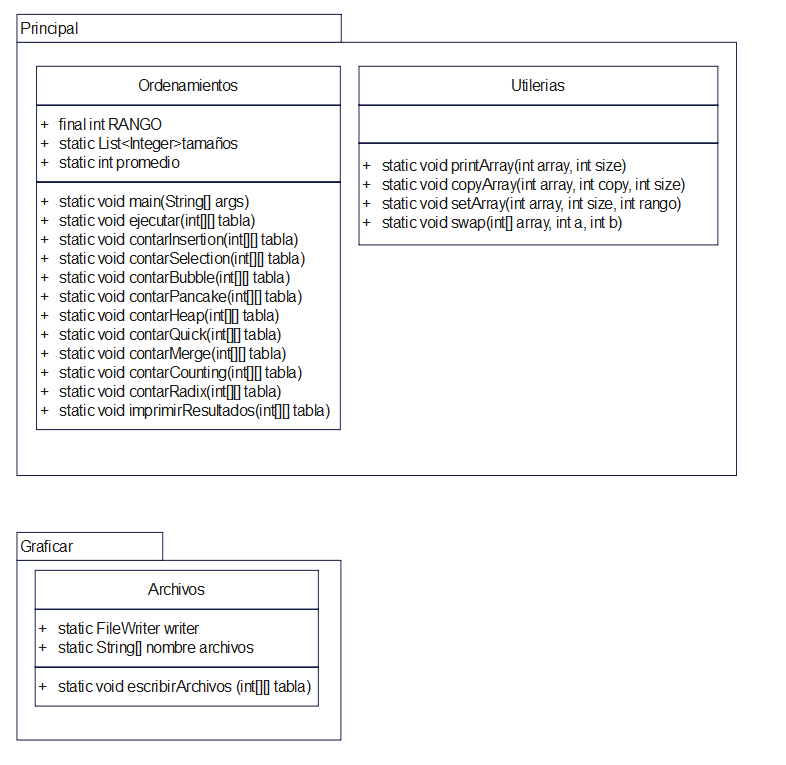
\includegraphics[width=1\textwidth]{media/UML1.PNG} 
\end{figure}

\begin{figure}[h] 
    \centering
    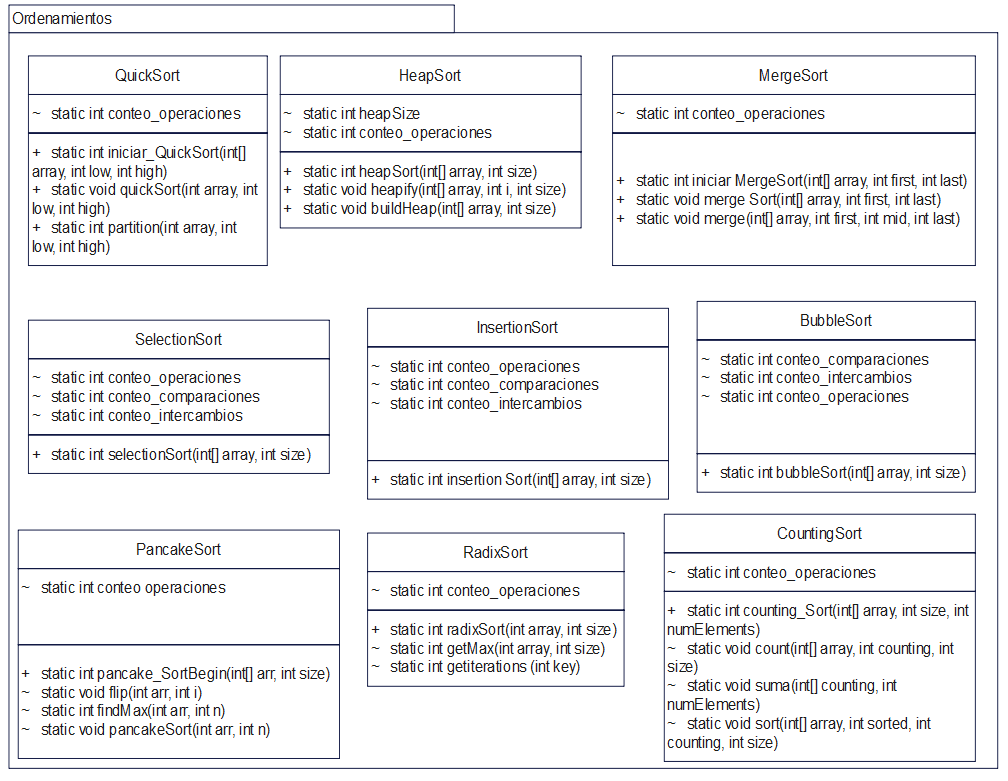
\includegraphics[width=1\textwidth]{media/UML2.PNG} 
\end{figure}


\newpage
\section{Bitácora del proyecto}

Regisro de fecha, hora y lugar/medio de reunión de los integrantes para la organización, asignación de tareas y discución del proyecto.\\

\begin{itemize}
    \item \textbf{Viernes 08 de marzo - 19:00 Hrs.}: Reunión en Zoom. Se estructuró de manera general lo que conformaría la realicación del proyecto, y se distribuyeron algunos puntos a trabajar.\\
    \textbf{Encargado(s)}: Cabrera Rojas Oscar, Chavez Marquez Sergio Antonio, Noyola Torres Pablo Sebastian.
    
    \item \textbf{Sábado 09 de marzo - 20:00 Hrs.}: Creación del archivo colaborativo de java, en la plataforma de \textit{Replit}. \\
    \textbf{Encargado(s)}: Noyola Torres Pablo Sebastian
    
    \item \textbf{Martes 12 de marzo - 20:00 Hrs.}: Implemetación individual de los ocho algoritmos de ordenamiento tratados en clase.\\
    Prueba individual en crudo. \\
    \textbf{Encargado(s)}: Cabrera Rojas Oscar

    \item \textbf{Martes 12 de marzo - 20:00 Hrs.}: Creación de los \textit{Archivos.java} y \textit{Graficar.py} para implementar la graficación de resultados posteriores a cada ejecución del programa principal. \\
    \textbf{Encargado(s)}: Cabrera Rojas Oscar
    
    \item \textbf{Jueves 14 de marzo - 06:00 Hrs.}: Implementación del algoritmo adicional (\textit{PancakeSort}). \\
    \textbf{Encargado(s)}: Noyola Torres Pablo Sebastian
    
    \item \textbf{Jueves 14 de marzo - 17:30 Hrs.}: Inicialicación y estructuración del archivo escrito en \LaTeX. \\
    \textbf{Encargado(s)}: Chavez Marquez Sergio Antonio

    \item \textbf{Jueves 14 de marzo - 19:00 Hrs.}: Implementación de contadores de operaciones \textit{BubbleSort}, \textit{SelectionSort} e \textit{InsertionSort}. \\
    \textbf{Encargado(s)}: Noyola Torres Pablo Sebastian

    \item \textbf{Jueves 14 de marzo - 22:00 Hrs.}: Organización en paquetes de las clases del programa. \\
    Implementación del algoritmo adicional (\textit{PancakeSort}) en la lógica de graficación. Planeación de la lógica del funcionamiento.\\
    \textbf{Encargado(s)}: Cabrera Rojas Oscar.

    \item \textbf{Jueves 15 de marzo - 22:00 Hrs.}: Organización y seleccionamiento de los contenidos textuales y de los archivos escritos en el procesador de \LaTeX mediante \textit{OverLeaf} correspondiente: trabajo\_escrito.tex y documentacion.text. \\
    \textbf{Encargado(s)}: Cabrera Rojas Oscar

    \item \textbf{Viernes 22 de marzo - 20:00 Hrs.}: Implementación de los contadpres en los algoritmos restantes, así como la rectificaión de los ya existentes. \\
    \textbf{Encargado(s)}: Chavez Marquez Sergio Antonio, Noyola Torres Pablo Sebastian.

    \item \textbf{Viernes 22 de marzo - 20:00 Hrs.}: Desarrollo final del programa principal \textit{Ordenamientos.java} y lógica de su funcionamiento terminada.\\
    \textbf{Encargado(s)}: Cabrera Rojas Oscar.

    \item \textbf{Viernes 22 de marzo - 22:00 Hrs.}: Desarrollo final del sistema de escritura y lectura de archivos de texto, cambios en \textit{Archivos.java} y \textit{Graficar.py}.\\
    \textbf{Encargado(s)}: Cabrera Rojas Oscar.

    \item \textbf{Sábado 23 de marzo - 00:30 Hrs.}: Reunión en Zoom. Primeras pruebas preliminares del funcionamiento del programa.\\
    \textbf{Encargado(s)}: Cabrera Rojas Oscar, Chavez Marquez Sergio Antonio, Noyola Torres Pablo Sebastian.

    \item \textbf{Sábado 23 de marzo - 10:00 Hrs.}: Reunión en Zoom. Corrección de variables contadoras de operaciones en \textit{QuickSort} y \textit{MergeSort}. Resolución de problema de retorno \textit{int} con recursividad.\\
    \textbf{Encargado(s)}: Cabrera Rojas Oscar, Chavez Marquez Sergio Antonio, Noyola Torres Pablo Sebastian.

    \item \textbf{Sábado 23 de marzo - 15:00 Hrs.}: Creación del programa \textit{GraficarLogaritmo.py} para realizar pruebas sobre el funcionamiento de graficación con Python y visualización de la forma de la gráfica $n\log(n)$\\
    \textbf{Encargado(s)}: Cabrera Rojas Oscar.

    \item \textbf{Sábado 23 de marzo - 22:00 Hrs.}: Cambio no planeado a \textit{Ordenamientos.java} para que la lista (antes arreglo) de tamaños sea dinámica y creada a partir de la entrada del usuario.\\
    \textbf{Encargado(s)}: Cabrera Rojas Oscar.

    \item \textbf{Domingo 24 de marzo - 20:00 Hrs.}: Reunión en Zoom. Organización para la grabación del video, y realización de pruebas.\\
    \textbf{Encargado(s)}: Cabrera Rojas Oscar, Chavez Marquez Sergio Antonio, Noyola Torres Pablo Sebastian.

    \item \textbf{Domingo 24 de marzo - 21:00 Hrs.}: Reunión en Zoom. Grabación conjunta del video explicativo sobre el funcionamiento del programa.\\
    \textbf{Encargado(s)}: Cabrera Rojas Oscar, Chavez Marquez Sergio Antonio, Noyola Torres Pablo Sebastian.

    \item \textbf{Lunes 25 de marzo - 02:00 Hrs.}: Edición del video explicativo sobre el funcionamiento del programa y adición de las pistas de audio individuales.\\
    \textbf{Encargado(s)}: Cabrera Rojas Oscar, Chavez Marquez Sergio Antonio, Noyola Torres Pablo Sebastian.

    \item \textbf{Lunes 25 de marzo - 22:00 Hrs.}: Terminamos el ingreso de la información en los archivos de texto correspondientes al ``Reporte Escrito'' y ``Documentación''.\\
    \textbf{Encargado(s)}: Cabrera Rojas Oscar, Chavez Marquez Sergio Antonio, Noyola Torres Pablo Sebastian.

\end{itemize}

\newpage
\section{Calendarización del proyecto}

Aquí se muestra un calendario del mes de marzo marcando los aspectos más relevantes de la cosntrucción de este proyecto.

\begin{figure}[h] 
    \centering
    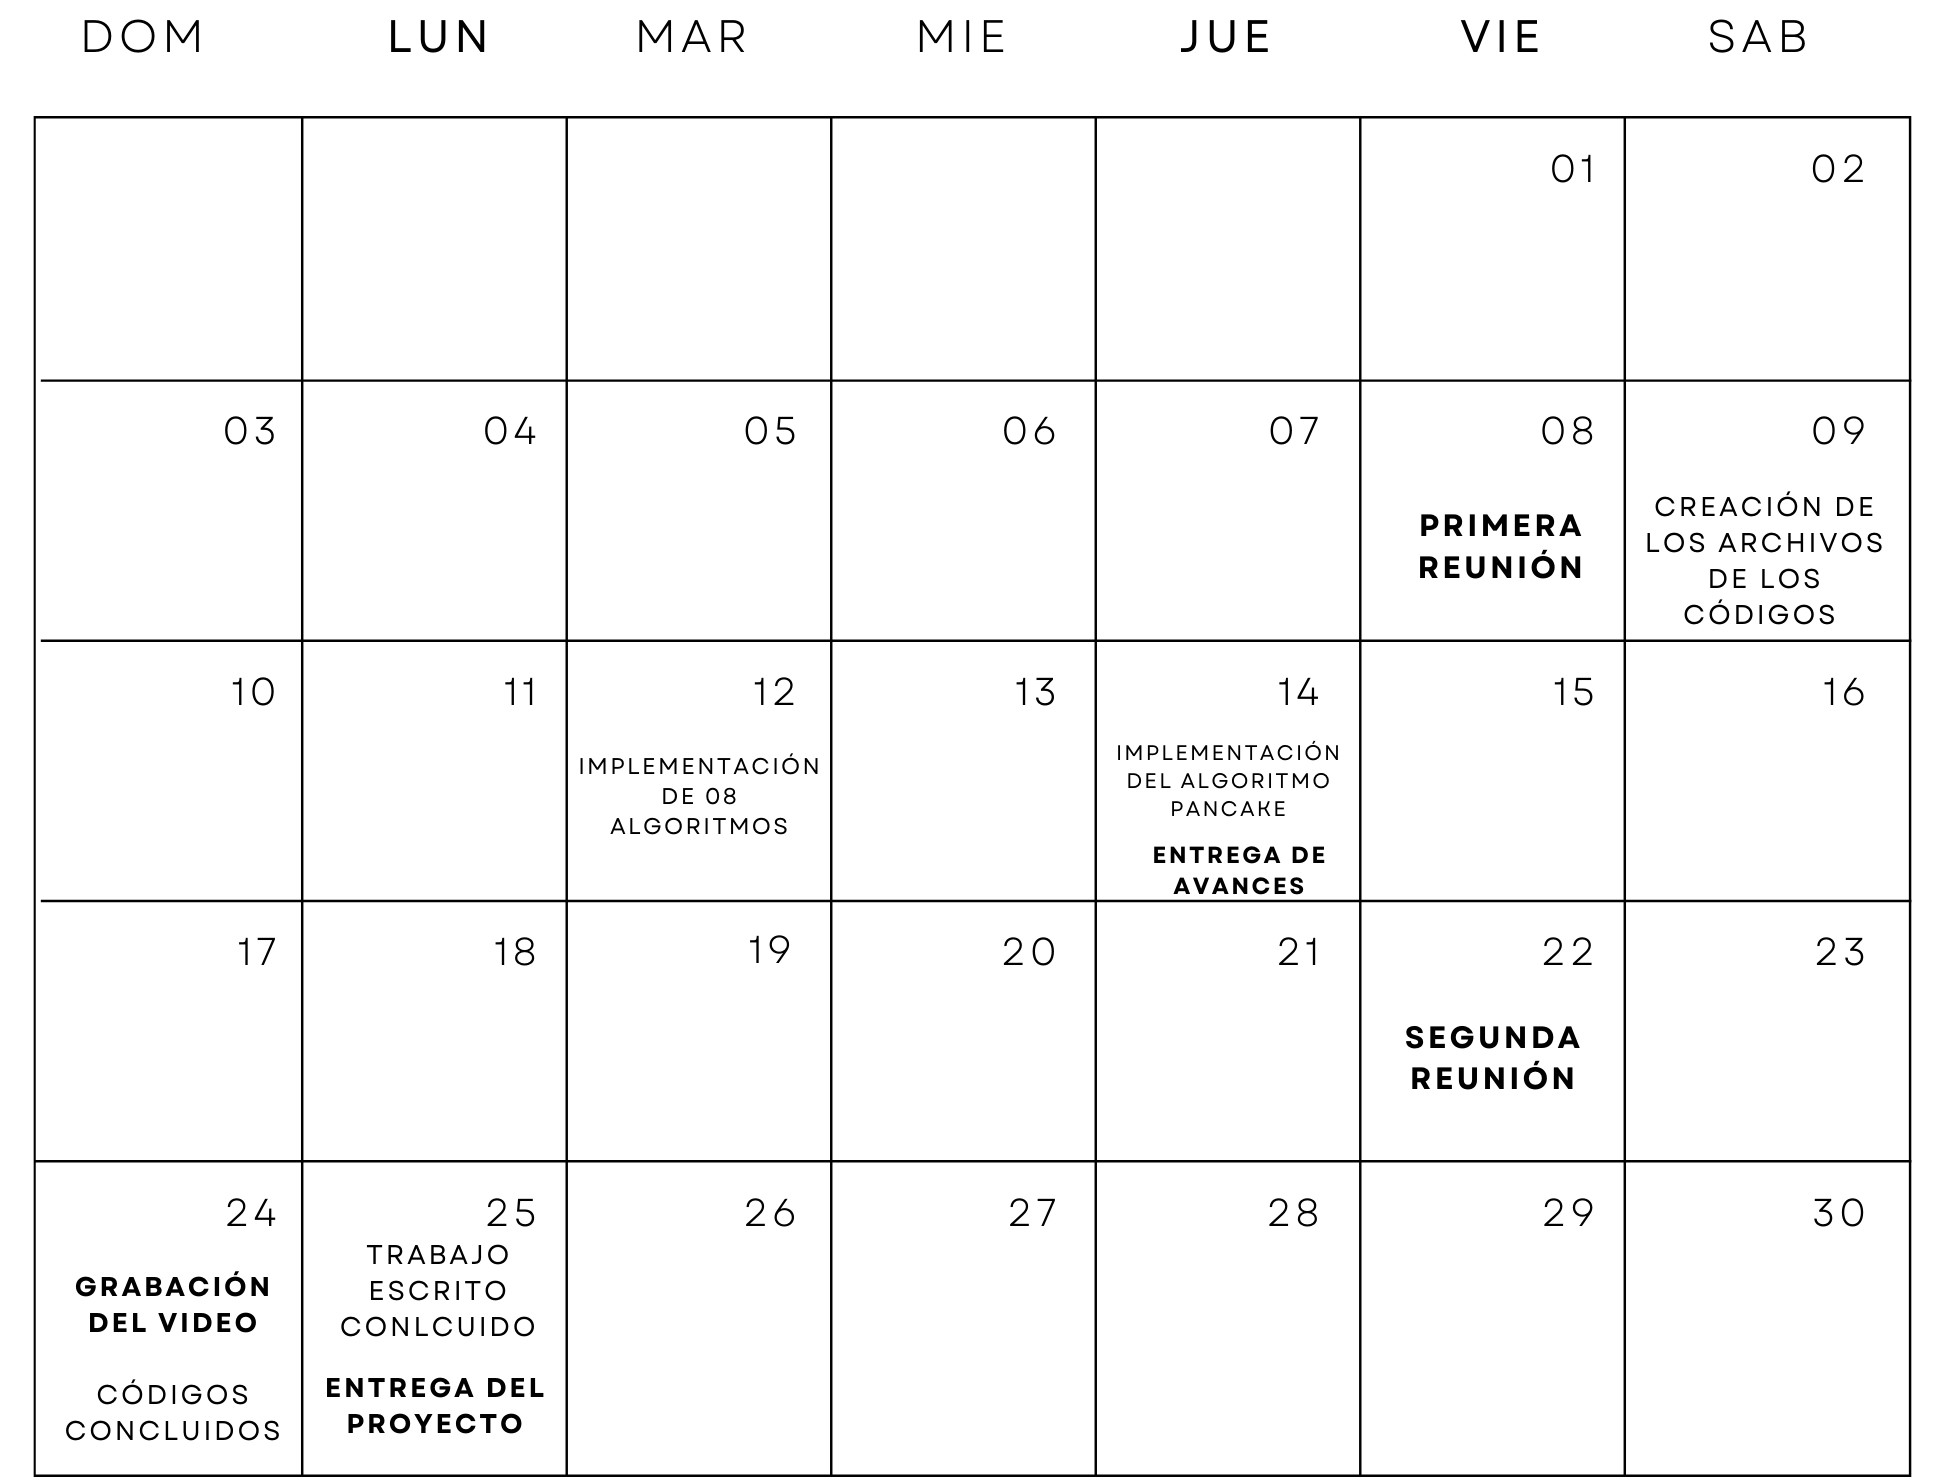
\includegraphics[width=1\textwidth]{media/Calendarizacion.jpg} 
\end{figure}


\end{document}
